\chapter{Test e validazione}
\label{cap:test}

\intro{In questo capitolo si espongono e discutono i test svolti su OpenVLC e sul modulo di autenticazione sviluppato. Il capitolo viene diviso in due sezioni: la prima riguarda i test svolti sul modulo di autenticazione sviluppato; la seconda riguarda test generici sul framework OpenVLC.}\\

% ================================================================= %
\section{Test sul modulo di autenticazione}
In questa sezione si riportano i risultati dei test svolti sul modulo di autenticazione sviluppato. L'obbiettivo di questi test è quello di analizzare le prestazioni di OpenVLC con l'utilizzo del modulo, confrontandole con quelle del framework OpenVLC originale. In più, si testa la qualità della comunicazione in diverse condizioni di luminosità ambientale: ambiente luminoso, ambiente buio e ambiente luminoso con disturbo indotto.

Sono stati condotti quattro test, ognuno della durata di circa 30 secondi. In tutti i test le schede sono state posizionate una di fronte all'altra ad una distanza di 100 centimetri. La comunicazione è stata testata utilizzando il comando \texttt{iperf}, il quale è un programma di misurazione delle prestazioni di rete. Si è scelto di utilizzare questo strumento anche per essere paragonabile ai test riportati nella documentazione di OpenVLC, anch'essi svolti con \texttt{iperf}.

In particolare, i comandi utilizzati per i test sono gli stessi riportati nella documentazione ufficiale di OpenVLC: per il trasmettitore "\texttt{sudo iperf -c 192.168.0.2 -u -b 400k -l 800 -p 10001 -t 100}"; mentre per il ricevitore "\texttt{sudo iperf -u -l 800 -s -i3 -B 192.168.0.2 -p 10001}".

\subsection{Descrizione dei test}

In figura \ref{fig:iperf_openvlc_originale}, si riporta il test iperf della documentazione di OpenVLC.
\begin{figure}[H] 
    \centering 
    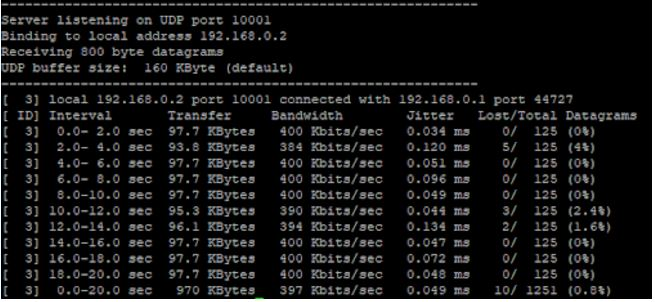
\includegraphics[width=0.9\columnwidth]{test/iperf_openvlc_originale} 
    \caption{Test iperf riportato nella documentazione di OpenVLC}
    \label{fig:iperf_openvlc_originale}
\end{figure}

\noindent In figura \ref{fig:iperf_openvlc_luce_ambiente}, si riporta il test iperf svolto in ambiente luminoso con OpenVLC originale. Si osserva che le differenze rispetto al test illustrato precedentemente, non sono statisticamente significative.
\begin{figure}[H] 
    \centering 
    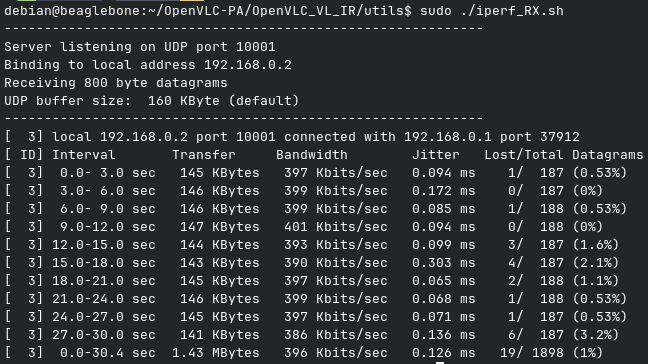
\includegraphics[width=0.9\columnwidth]{test/master_luce_ambiente} 
    \caption{Test iperf con OpenVLC in ambiente luminoso}
    \label{fig:iperf_openvlc_luce_ambiente}
\end{figure}

\noindent In figura \ref{fig:iperf_openvlc_auth_luce_ambiente}, si riporta il test iperf svolto in ambiente luminoso con OpenVLC e con l'utilizzo del modulo di autenticazione sviluppato.
\begin{figure}[H] 
    \centering 
    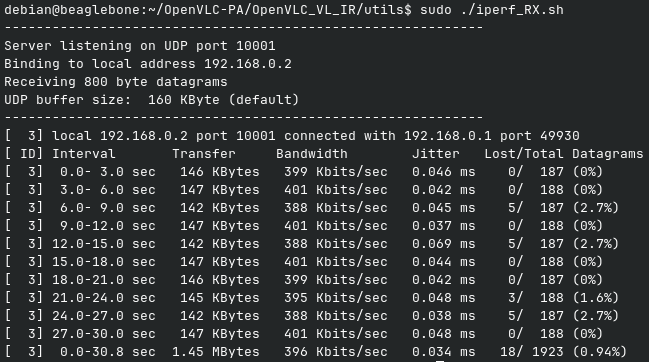
\includegraphics[width=0.9\columnwidth]{test/PhyAuth_luce_ambiente} 
    \caption{Test iperf con OpenVLC e modulo di autenticazione in ambiente luminoso}
    \label{fig:iperf_openvlc_auth_luce_ambiente}
\end{figure}

\noindent In figura \ref{fig:iperf_openvlc_auth_buio}, si riporta il test iperf svolto in ambiente buio con OpenVLC e con l'utilizzo del modulo di autenticazione sviluppato.
\begin{figure}[H] 
    \centering 
    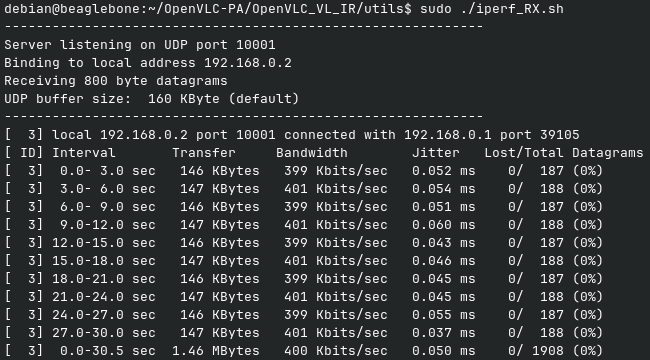
\includegraphics[width=0.9\columnwidth]{test/PhyAuth_buio} 
    \caption{Test iperf con OpenVLC e modulo di autenticazione in ambiente buio}
    \label{fig:iperf_openvlc_auth_buio}
\end{figure}

\noindent In figura \ref{fig:iperf_openvlc_auth_luce_disturbo}, si riporta il test iperf svolto in ambiente luminoso con OpenVLC e con l'utilizzo del modulo di autenticazione sviluppato. In più, in questo test è stato introdotto un disturbo luminoso, posizionando una lampada diretta verso il fotodiodo ricevitore ad una distanza di circa 20 centimetri. Tale disturbo è stato indotto per simulare un attacco di disturbo alla comunicazione, in modo tale da testare la robustezza della comunicazione.
\begin{figure}[H] 
    \centering 
    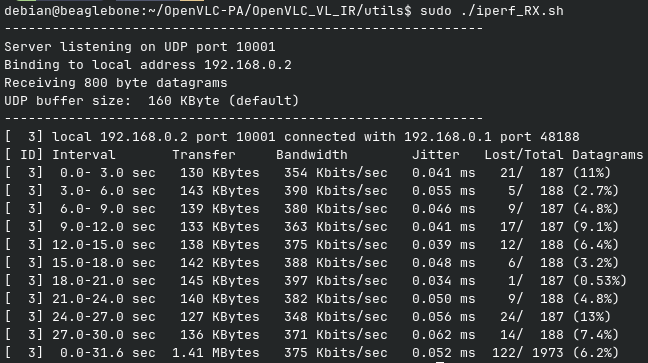
\includegraphics[width=0.9\columnwidth]{test/PhyAuth_luce_e_disturbo} 
    \caption{Test iperf con OpenVLC e modulo di autenticazione in ambiente luminoso con disturbo indotto}
    \label{fig:iperf_openvlc_auth_luce_disturbo}
\end{figure}

\subsection{Analisi dei risultati}

Nella seguente tabella si riassumono i risultati dei test descritti nella precedente sezione. I dati sono ricavati dall'ultima riga di ogni test, che rappresenta il valore medio delle metriche calcolate nell'intervallo di tempo in cui si è svolta la comunicazione.
\begin{table}[H]
    \caption{Tabella riassuntiva dei risultati dei test sul modulo di autenticazione}
    \label{tab:riass-test-auth}
    \begin{tabularx}{\textwidth}{lllllc}
        \hline
        \textbf{Test} & \textbf{Interval} & \textbf{Transfer} & \textbf{Bandwidth} & \textbf{Jitter} & \textbf{Lost/Total}\\
        \hline
        OpenVLC\\in ambiente\\luminoso & 30.4 sec & 1.43 MBytes & 396 Kbits/sec & 0.126 ms & 19/1898 (1\%) \\
        \hline
        OpenVLC\\+ modulo\\in ambiente\\luminoso & 30.8 sec & 1.45 MBytes & 396 Kbits/sec & 0.034 ms & 18/1923 (0.94\%) \\
        \hline
        OpenVLC\\+ modulo\\in ambiente\\buio & 30.5 sec & 1.46 MBytes & 400 Kbits/sec & 0.050 ms & 0/1988 (0\%) \\
        \hline
        OpenVLC\\+ modulo\\in ambiente\\luminoso\\con disturbo & 31.6 sec & 1.41 MBytes & 375 Kbits/sec & 0.052 ms & 122/1973 (6.2\%) \\
        \hline
    \end{tabularx}
\end{table}

\noindent Come si può osservare dalle prime due righe della tabella \ref{tab:riass-test-auth}, a parità di condizioni ambientali, non c'è alcuna differenza sistematicamente significativa tra le prestazioni del sistema con e senza l'utilizzo del modulo di autenticazione. Le lievi differenze presenti sono infatti da interpretarsi come rumore. Di conseguenza si può affermare che la sua introduzione non ha un impatto rilevante sulle prestazioni del sistema.

Si possono invece notare differenze significative tra i test svolti in ambiente luminoso e quelli svolti in divese condizioni di luminosità.\\
In particolare, il test svolto in ambiente buio ha mostrato un'ampiezza di banda (bandwidth) e un tasso di perdita migliori rispetto a quelli svolti in ambiente luminoso. Questo suggerisce che la comunicazione tramite luce visibile, seppure in maniera minima, trattandosi di una variazione dell'1\%, è sicuramente influenzata dalla presenza di luce ambientale.\\
Inoltre, il test svolto in ambiente luminoso con disturbo indotto ha mostrato un tasso di perdita notevolmente più alto rispetto agli altri test, pari al 6.2\%. Si deduce che la presenza di fonti luminose dirette in direzione del fotodiodo ricevitore, sono in grado di disturbare notevolmente la comunicazione. Tuttavia è importante evidenziare che la situazione in cui è stato testato il sistema, e cioè posizionando una fonte luminosa a distanza molto ravvicinata al fotodiodo, è estrema. Di conseguenza, resta particolarmente difficoltoso, per un potenziale attaccante che volesse disturbare la ricezione dei dati, farlo in questa maniera.

% ================================================================= %
\section{Test su OpenVLC}
In questa sezione si riportano i risultati dei test svolti sul framework OpenVLC originale, cioè senza l'utilizzo del modulo di autenticazione sviluppato. L'obbiettivo di questi test è quello di analizzare le prestazioni di OpenVLC a diverse distanze ed inclinazioni.

Sono stati condotti nove test, in ognuno dei quali sono stati trasmessi 1000 pacchetti di dati tramite il comando \texttt{nc} (netcat), ognuno della dimensione di 1480 byte. In tutti i test il payload era formato da byte "FF", ovvero da 8 bit impostati a "1", in modo tale da poter individuare efficacemente eventuali bit corrotti. L'unica eccezione è il test denominato "50 cm bit-0", in cui il payload era formato da byte "00", ovvero da 8 bit impostati a "0", per poter osservare eventuali bias a favore di bit-0 piuttosto che bit-1.

Tutti i test sono stati svolti in ambiente luminoso e senza l'utilizzo di Reed-Solomon, in modo tale da poter osservare le prestazioni del canale fisico senza l'intervento di alcun protocollo di correzione degli errori.

Inoltre, c'è da precisare che le schede BeagleBone non dispongono di una capacità computazionale elevata, di conseguenza il solo fatto di osservare la comunicazione e salvarne i dati, rende le schede maggiormente soggette ad errori. Questo implica che le metriche di errore calcolate durante i test sono sovrastimate rispetto a quelle che il sistema raggiunge in condizioni normali.\\

\noindent I test vengono valutati utilizzando le seguenti metriche:
\begin{itemize}
    \item Bit Error Rate (BER): rapporto tra il numero di bit ricevuti in errore e il numero totale di bit trasmessi, indicativo dell’affidabilità a livello fisico del canale.
    \item Percentuale di byte corrotti: percentuale di byte che contengono almeno un bit errato rispetto al totale dei byte trasmessi, utile per valutare la possibilità di correggere errori con Reed-Solomon.
    \item Packet Reception Rate (PRR): frazione di pacchetti correttamente ricevuti sul numero di pacchetti inviati, misura l’efficacia complessiva del link.
    \item Packet Loss Rate (PLR): percentuale di pacchetti persi rispetto al totale inviato; è il complementare di PRR.
    \item Percentuale di payload ricevuto: rapporto tra il numero di byte di payload validi ricevuti e il numero di byte di payload trasmessi, espressa in percentuale, per quantificare l’efficienza utile della trasmissione.
\end{itemize}

\subsection{Descrizione dei test}
Come accennato in precedenza, sono stati condotti nove test, tutti in ambiente luminoso.

L'unico test in cui il payload era formato da byte "00" è il test denominato "50 cm bit-0", in cui le schede sono state posizionate una di fronte all'altra ad una distanza di 50 centimetri. In tutti gli altri il payload era formato da byte "FF".

Nei test denominati "50 cm bit-1", "100 cm", "150 cm", "200 cm", le schede sono state posizionate perfettamente allineate una di fronte all'altra ad una distanza di 50, 100, 150 e 200 centimetri rispettivamente.

Nei test denominati "50 cm 10°", "50 cm 45°", "50 cm 60°", "50 cm 90°", le schede sono state posizionate ad una distanza di 50 centimetri, ma con un'inclinazione di 10°, 45°, 60° e 90° rispettivamente. Ovvero per ogni inclinazione, la scheda trasmittente è stata ruotata, rispetto alla scheda ricevente, di un angolo corrispondente, mantenendo la stessa distanza.

\subsection{Analisi dei risultati}
\subsubsection{Bias a favore di bit-0}
Per prima cosa, è necessario confrontare i test "50 cm bit-0" e "50 cm bit-1", in modo tale da osservare se vi è un bias a favore di bit-0 rispetto a bit-1. In tabella \ref{tab:bit-bias} sono riportate le metriche di errore calcolate per i due test.

Nonostante, a prima vista, la differenza in tutte le metriche sembrerebbe minima, è importante considerare che la numerosità dei campioni è di diversi milioni di bit. Di conseguenza, anche una piccola differenza può essere considerata statisticamente significativa.

Si osserva che le uniche metriche che non presentano una differenza significativa sono il Packet Reception Rate (PRR) e il Packet Loss Rate (PLR). Il che denota, come ci si aspetterebbe date le pari condizioni ambientali in cui sono stati svolti i test, che in entrambi i casi le schede riescono a sincronizzarsi correttamente.

Tuttavia, si osserva che il Bit Error Rate (BER) è più basso per i bit-0 rispetto ai bit-1, con un valore di 1.10\% per i bit-0 e di 1.25\% per i bit-1. Inoltre, la percentuale di byte corrotti è più alta per i bit-1 (2.56\%) rispetto ai bit-0 (1.93\%). Infine, la percentuale di payload ricevuto è più alta per i bit-0 (99.24\%) rispetto ai bit-1 (95.83\%). Questo indica che i bit-1 tendono a essere corrotti più frequentemente rispetto ai bit-0, il che suggerisce un bias a favore dei bit-0.

La presenza di questo bias comporta che le metriche di errore calcolate per i successivi test, in quanto basati su bit-1, sono da considerarsi sovrastimate. In una normale comunicazione, ci si aspetta un bilanciamento tra i bit-0 e i bit-1, e di conseguenza che le metriche di errore siano comprese tra i valori di errore dei bit-0 e dei bit-1 qui presentati.

\begin{table}[H]
    \caption{Confronto delle metriche di errore di bit-0 e bit-1: bias a favore di bit-0}
    \label{tab:bit-bias}
    \begin{tabularx}{\textwidth}{Xll}
        \hline
        \textbf{Metrica} & \textbf{50 cm bit-0} & \textbf{50 cm bit-1}\\
        \hline
        Bit Error Rate (BER)            & 1.10\%  & 1.25\% \\
        \hline
        \% Byte corrotti                & 2.56\%  & 1.93\% \\
        \hline
        Packet Reception Rate (PRR)     & 93.80\% & 93.90\% \\
        \hline
        Packet Loss Rate (PLR)          & 6.20\%  & 6.10\% \\
        \hline
        \% Payload Ricevuto             & 99.24\% & 95.83\% \\
        \hline
    \end{tabularx}
\end{table}

\subsubsection{Test a diverse distanze}
% TODO

\subsubsection{Test a diverse inclinazioni}
